\documentclass[12pt,a4paper]{article}
\usepackage[utf8]{inputenc}
\usepackage[T1]{fontenc}
\usepackage[english]{babel}
\usepackage{lmodern}
\usepackage{microtype}
\usepackage{amsmath, amssymb, amsfonts}
\usepackage[margin=2.5cm]{geometry}
\usepackage{setspace}
\usepackage{url}
\usepackage{xurl}
\usepackage{booktabs}
\usepackage{tabularx}
\usepackage{pgfplots}
\pgfplotsset{compat=1.18}
\usetikzlibrary{babel}

\onehalfspacing

\title{\textbf{Stationary Strings Theorem VIII: Falsifiable Predictions, 511 keV Spectral Band, and Uncertainty Quantification} \\[0.3cm]
\large (BASE-STEP 136 mT Sideband Falsification, ALPHA 1.05 T Third-Field Prediction, Exact 1949 Ore--Powell Photon Budget, and Independent Cross-Check)}
\author{Fahri Meral}
\date{October 17, 2026}

\begin{document}

\maketitle

\begin{abstract}
As the falsification ring of the Theorems I--VII series, this 8th work converts the retrospective matches of the previous papers into prospective, refutable predictions:
\begin{enumerate}
    \item BASE-STEP 136 mT weak-field pair: the Theorem 5 Lyapunov potential predicts the centered+protected start locks at $r_-^{\mathrm{end}} = 1.1167668233\,\mu\text{m}$, $1$--$4\text{ mm}$ offsets recapture to the same point within 24 minutes, and the unprotected arm ($\mu_s=0$) hits the wall (\textbf{Test T20}).
    \item ALPHA third-field prediction: at $B_3=1.05\text{ T}$ the drift is locked by Eq.\ (\ref{eq:t21pred}); the $R(1.05/1.03)$ and $R(1.07/1.05)$ ratios are written down beforehand (\textbf{Test T21}).
    \item 511 keV spectral budget: via the exact 1949 Ore--Powell form, the $R = r_{\mathrm{oPs}}/r_{\mathrm{Line}}$ value ($f_{\mathrm{Ps}}=0.92$), the $f_{\mathrm{Ps}}\in[0.90,0.94]$ band, and the $P_s=1$ thermalized-island budget are predicted (\textbf{Test T22}).
\end{enumerate}
Uncertainty quantification (UQ) of four lock outputs and an independent 7-point cross-check that never imports the solver close the chain. The numerical chain closes at \texttt{T1--T22 (22/22 PASS)}.
\end{abstract}

\section{Introduction and Model--Source Separation (Honesty Framework)}

Stationary Strings Theorems I--VII [1--7] arrested the vortex singularity, derived Dirac--Majorana peeling and the $\Lambda_{\mathrm{Meral}}$ constant, and resolved the CERN ALPHA/BASE-STEP trap problems and the 511 keV spectrum. This work is different: it converts the previous matches into \textbf{prospective, refutable predictions} and puts the series' self-auditing discipline on record.

\textbf{Model--source separation:} the 136 mT envelope equation, the third-field ratio lock, the photon-budget band, and the UQ sensitivities are this work's \textit{theoretical model construction}; the BASE-STEP $136\text{ mT}$ campaign data, the ALPHA $1.03/1.07\text{ T}$ drifts and ECR measurements [8,9], $f_{\mathrm{Ps}}=0.92$ and $P_{\mathrm{surv}}\in[0.81,0.96]$ [10] are directly verified \textit{experimental/observational data}.

\textbf{Correction note (solver proton constant):} the independent cross-check caught the code's Breit--Rabi proton constant written $1000\times$ wrong ($\mu_{N}/h = 7.62\times 10^9$ instead of $7.62\times 10^6\text{ Hz/T}$) and it was corrected. Absolute $f_{da}/f_{cb}$ frequencies were $\sim 10.5\text{ MHz}$ off; the Breit--Rabi \textbf{slopes} changed by only 0.04\% ($28.0182\to 28.0080\text{ GHz/T}$). The T15 $f_{da}-f_{cb}=a_{1S}$ invariant was never affected by common-mode cancellation; Paper VII results stand. The T17/T21 numbers below are recomputed with the corrected slope.

\section[Task 15 / Test T20 --- BASE-STEP 136 mT Sideband On/Off Falsification]{Task 15 / Test T20 --- BASE-STEP 136 mT Sideband On/Off Falsification}

The $V_{\mathrm{well}}=16.0\text{ V}$-scaled axial frequency $\nu_z=0.916251\text{ MHz}$ gives, at $B_0=0.136\text{ T}$, $\nu_+=1.845952\text{ MHz}>\nu_z>\nu_-=227.393594\text{ kHz}>0$ (Table~\ref{tab:t20}). The analytic fixed point of the Theorem 5 envelope equation is $r^*=1.1167668231\,\mu\text{m}$ (brentq); the 24-minute Radau evolution settles the centered start at $r_-^{\mathrm{end}}=1.1167668233\,\mu\text{m}$ (Figure~\ref{fig:fig10}(a)). All $r_0=1,2,3,4\text{ mm}$ offsets recapture to the same point; the unprotected arm ($\mu_s=0$, $1\,\mu\text{m}$ seed) hits the wall. The prediction is sharp: \textbf{in the 136 mT campaign, loss starts with sideband cooling off and does not start with it on.} The high-field pairs show the same structure: centered $r_-^{\mathrm{end}}=0.1725929420\,\mu\text{m}$ at $0.880\text{ T}$ ($2/4\text{ mm}$ offsets recaptured, unprotected lost) and $r_-^{\mathrm{end}}=0.1529524641\,\mu\text{m}$ at $0.993\text{ T}$ (offsets recaptured, unprotected lost).

\begin{table}[!htbp]
\centering
\footnotesize
\setlength{\tabcolsep}{3pt}
\caption{\textbf{BASE-STEP 136 mT Weak-Field Falsification Pair} (Test T20, $t=1440\text{ s}$).}
\label{tab:t20}
\vspace{0.1cm}
\begin{tabular}{@{}l|c@{}}
\hline
Quantity & Value \\
\hline
$\nu_c$ / $\nu_+$ / $\nu_z$ / $\nu_-$ ($0.136$ T, $16$ V) & $2.073$ / $1.846$ / $0.916$ MHz / $227.394$ kHz \\
Analytic fixed point $r^*$ ($\mu_s^*$) & $1.1167668231\,\mu\text{m}$ \\
Centered+protected $r_-^{\mathrm{end}}(24\text{ min})$ & $1.1167668233\,\mu\text{m}$ \\
Offsets $r_0=1/2/3/4\text{ mm}$ $\to$ $r_-^{\mathrm{end}}$ & $1.1167668233\,\mu\text{m}$ (all recaptured) \\
Unprotected ($\mu_s=0$) $r_-(24\text{ min})$ & $>5.0$ mm (wall loss) \\
High-field pair ($0.880/0.993$ T) centered $r_-^{\mathrm{end}}$ & $0.1725929420$ / $0.1529524641\,\mu\text{m}$ \\
(offsets recaptured, unprotected lost) & \\
Fragility: critical $\mu_s$ band / $\mu_s=0.10$ marginal $r^*$ & $[0.05, 0.15]$ / $90.5544376963\,\mu\text{m}$ ($<0.5$ mm) \\
\hline
\end{tabular}
\end{table}

\section{Task 16 / Test T21 --- ALPHA 1.05 T Third-Field Prediction and Ratio Lock}

With the $1.03/1.07\text{ T}$ gamma mean $\bar{\gamma}=7.0112543975\times 10^{-10}\text{/s}$ (relative spread $1.49\times 10^{-4}$) and the corrected $\partial f_{da}/\partial B(1.05\text{ T})=28.0086802081\text{ GHz/T}$ (Table~\ref{tab:t21}, Figure~\ref{fig:fig10}(b)):
\begin{equation}
\boxed{\dot{f}_{\mathrm{pred}}(1.05\text{ T}) = -74.2301213010 \pm 0.0055473080\text{ kHz/h}}
\label{eq:t21pred}
\end{equation}
and the ratio locks $R(1.05/1.03)=1.0194406565$, $R(1.07/1.05)=1.0190695066$ are written down in advance. Retrospective methodology validation (leave-one-out): $1.03$-only prediction of $1.07$ gives $-75.651306$ ($149.5\text{ ppm}$ error), $1.07$-only prediction of $1.03$ gives $-72.809117$ ($149.5\text{ ppm}$). A future $1.05\text{ T}$ measurement outside this band falsifies the ratio law.

\begin{table}[!htbp]
\centering
\footnotesize
\setlength{\tabcolsep}{3pt}
\caption{\textbf{ALPHA Third-Field Frequency-Drift Prediction} (Test T21, $B_3=1.05\text{ T}$).}
\label{tab:t21}
\vspace{0.1cm}
\begin{tabular}{@{}l|c@{}}
\hline
Quantity & Value \\
\hline
$\partial f_{da}/\partial B(1.05\text{ T})$ & $28.0086802081$ GHz/T \\
$\dot{f}_{\mathrm{pred}}(1.05\text{ T})$ & $-74.2301213010 \pm 0.0055473080$ kHz/h \\
$R(1.05/1.03)$ / $R(1.07/1.05)$ & $1.0194406565$ / $1.0190695066$ \\
LOO ($1.03\to1.07$ / $1.07\to1.03$) & $149.5$ / $149.5\text{ ppm}$ \\
$\bar{\gamma}$ relative spread & $1.4946245170\times 10^{-4}$ \\
\hline
\end{tabular}
\end{table}

\section{Task 17 / Test T22 --- 511 keV Photon-Budget Prediction Band}

The Siegert--Yoneda [10] photon-count algebra ($r_{\mathrm{Line}}=P_{\mathrm{surv}}(2-\frac32f_{\mathrm{Ps}})$, $r_{\mathrm{oPs}}=P_{\mathrm{surv}}\frac94f_{\mathrm{Ps}}$) combined with the exact 1949 $O_{\mathrm{exact}}$ (Table~\ref{tab:t22}, Figure~\ref{fig:fig10}(c)):
\begin{equation}
\boxed{R = \frac{r_{\mathrm{oPs}}}{r_{\mathrm{Line}}} = 3.3387096774 \quad (f_{\mathrm{Ps}} = 0.92)}
\label{eq:t22R}
\end{equation}
with the $f_{\mathrm{Ps}}\in[0.90,0.94]$ band $[3.1153846154, 3.5847457627]$. On the $P_s=1$ thermalized island the exact budget is $0.62$ (line) $+2.07$ (o-Ps) $=2.6900000000$ (numerical closure $1.07\times 10^{-14}$); under partial thermalization the in-flight leak $2(1-P_s)\le 0.38$ is reported as a separate upper bound. The line centroid is identically $511.0\text{ keV}$. SPI region map (Churazov et al.\ 2005, Weidenspointner et al.\ 2006, Jean et al.\ 2006 compilation [17--19]): Bulge $f_{\mathrm{Ps}}=0.92\pm0.02$ (calibration point, $0.00\sigma$), Disk $f_{\mathrm{Ps}}=0.91\pm0.02$ ($R=3.2244094488\pm0.223$, $0.51\sigma$ independent test), Halo $f_{\mathrm{Ps}}=0.65\pm0.07$ ($R=1.4268292683$, $6.38\sigma$ off-band --- sparse-gas in-flight regime, predicted as outside the model's validity).

\begin{table}[!htbp]
\centering
\footnotesize
\setlength{\tabcolsep}{3pt}
\caption{\textbf{511 keV Photon-Budget Prediction Band} (Test T22, exact 1949 $O_{\mathrm{exact}}$).}
\label{tab:t22}
\vspace{0.1cm}
\begin{tabular}{@{}l|c@{}}
\hline
Quantity & Value \\
\hline
$R = r_{\mathrm{oPs}}/r_{\mathrm{Line}}$ ($f_{\mathrm{Ps}}=0.92$) & $3.3387096774$ \\
Band ($f_{\mathrm{Ps}}\in[0.90,0.94]$) & $[3.1153846154, 3.5847457627]$ \\
$P_s=1$ budget (line $+$ o-Ps) & $0.62 + 2.07 = 2.6900000000$ ($1.07\times 10^{-14}$) \\
In-flight leak upper bound & $2(1-0.81) = 0.38$ \\
Line centroid & $511.0$ keV \\
COSI-2027 frame (threshold $10^{-6}$, 10/10 sources above) & $R$ band applies to all above-threshold sources \\
& $[3.1153846154, 3.5847457627]$ \\
SPI outer validation (Bulge fluxes, $\times10^{-4}$) & $R_{\mathrm{obs}}=3.1758241758\pm0.402$ \\
($28.9\pm2.9$ / $9.1\pm0.7$) vs.\ $R_{\mathrm{model}}=3.3387096774$ & ($0.41\sigma$ agreement) \\
SPI region map: Bulge / Disk / Halo & $0.00\sigma$ (calibr.) / $0.51\sigma$ / $6.38\sigma$ (IA) \\
\hline
\end{tabular}
\end{table}

\section{Uncertainty Quantification (UQ) and Independent Cross-Check}

Sensitivities of four lock outputs to input uncertainties (Figure~\ref{fig:fig10}(d), Table~\ref{tab:uq}): $r_p^{\mathrm{Meral}}|\mu_s$ sensitivity $0.8221385680$ (sub-linear); $R_{\mathrm{th}}$ derivative-step spread $45.9354534921\text{ ppm}$; $\dot{M}_{\mathrm{acc}}(\eta=0.10)=8.0016447377\times 10^{-8}\,M_\odot\text{/yr}$, spanning $[8.8907163753, 7.2742224889]\times 10^{-8}$ over $\eta\in[0.09,0.11]$ (exactly linear, $\pm 10\%$); $r^*(136\text{ mT})=1.1167781304\,\mu\text{m}$, spanning $[1.0051003173, 1.2284559434]\,\mu\text{m}$ over $a_{\mathrm{rms}}\pm 10\%$ ($\pm 10\%$). The spectral-ratio sensitivity $dR/df_{\mathrm{Ps}} = 72/(8-6f_{\mathrm{Ps}})^2 = 11.7065556712$ ($f_{\mathrm{Ps}}=0.92$) is consistent with the band width.

\begin{table}[!htbp]
\centering
\footnotesize
\setlength{\tabcolsep}{3pt}
\caption{\textbf{Lock-Output Sensitivities} (UQ, 1-sigma scale).}
\label{tab:uq}
\vspace{0.1cm}
\begin{tabular}{@{}l|c@{}}
\hline
Output $|$ input & Result \\
\hline
$r_p^{\mathrm{Meral}}|\mu_s$ & $0.8221385680$ (sub-linear) \\
$R_{\mathrm{th}}$ spread & $45.9354534921$ ppm \\
$\dot{M}_{\mathrm{acc}}|\eta\in[0.09,0.11]$ & $[8.8907163753, 7.2742224889]\times 10^{-8}\,M_\odot\text{/yr}$ \\
$r^*(136\text{ mT})|a_{\mathrm{rms}}\pm 10\%$ & $[1.0051003173, 1.2284559434]\,\mu\text{m}$ \\
$R|f_{\mathrm{Ps}}$ ($dR/df = 11.7065556712$) & $[3.1153846154, 3.5847457627]$ \\
$\Lambda_{\mathrm{Meral}}^{(0)}$ triple-path diff. & quad $0.0$ / trapz $6.39\times 10^{-10}$ / MC $1.05\times 10^{-4}$ \\
\hline
\end{tabular}
\end{table}

The independent mini-solver that never imports the solver (\path{duran_sicimler_sim/mini_check_viii.py}: hand-written uncoupled-basis Breit--Rabi, Simpson $\int O\approx 1$, explicit-Euler vs.\ brentq envelope, direct $r_p^{\mathrm{ideal}}$ evaluation) gives \textbf{7/7 PASS}; it was this chain that caught the proton-constant bug.

\begin{figure}[!htbp]
\centering
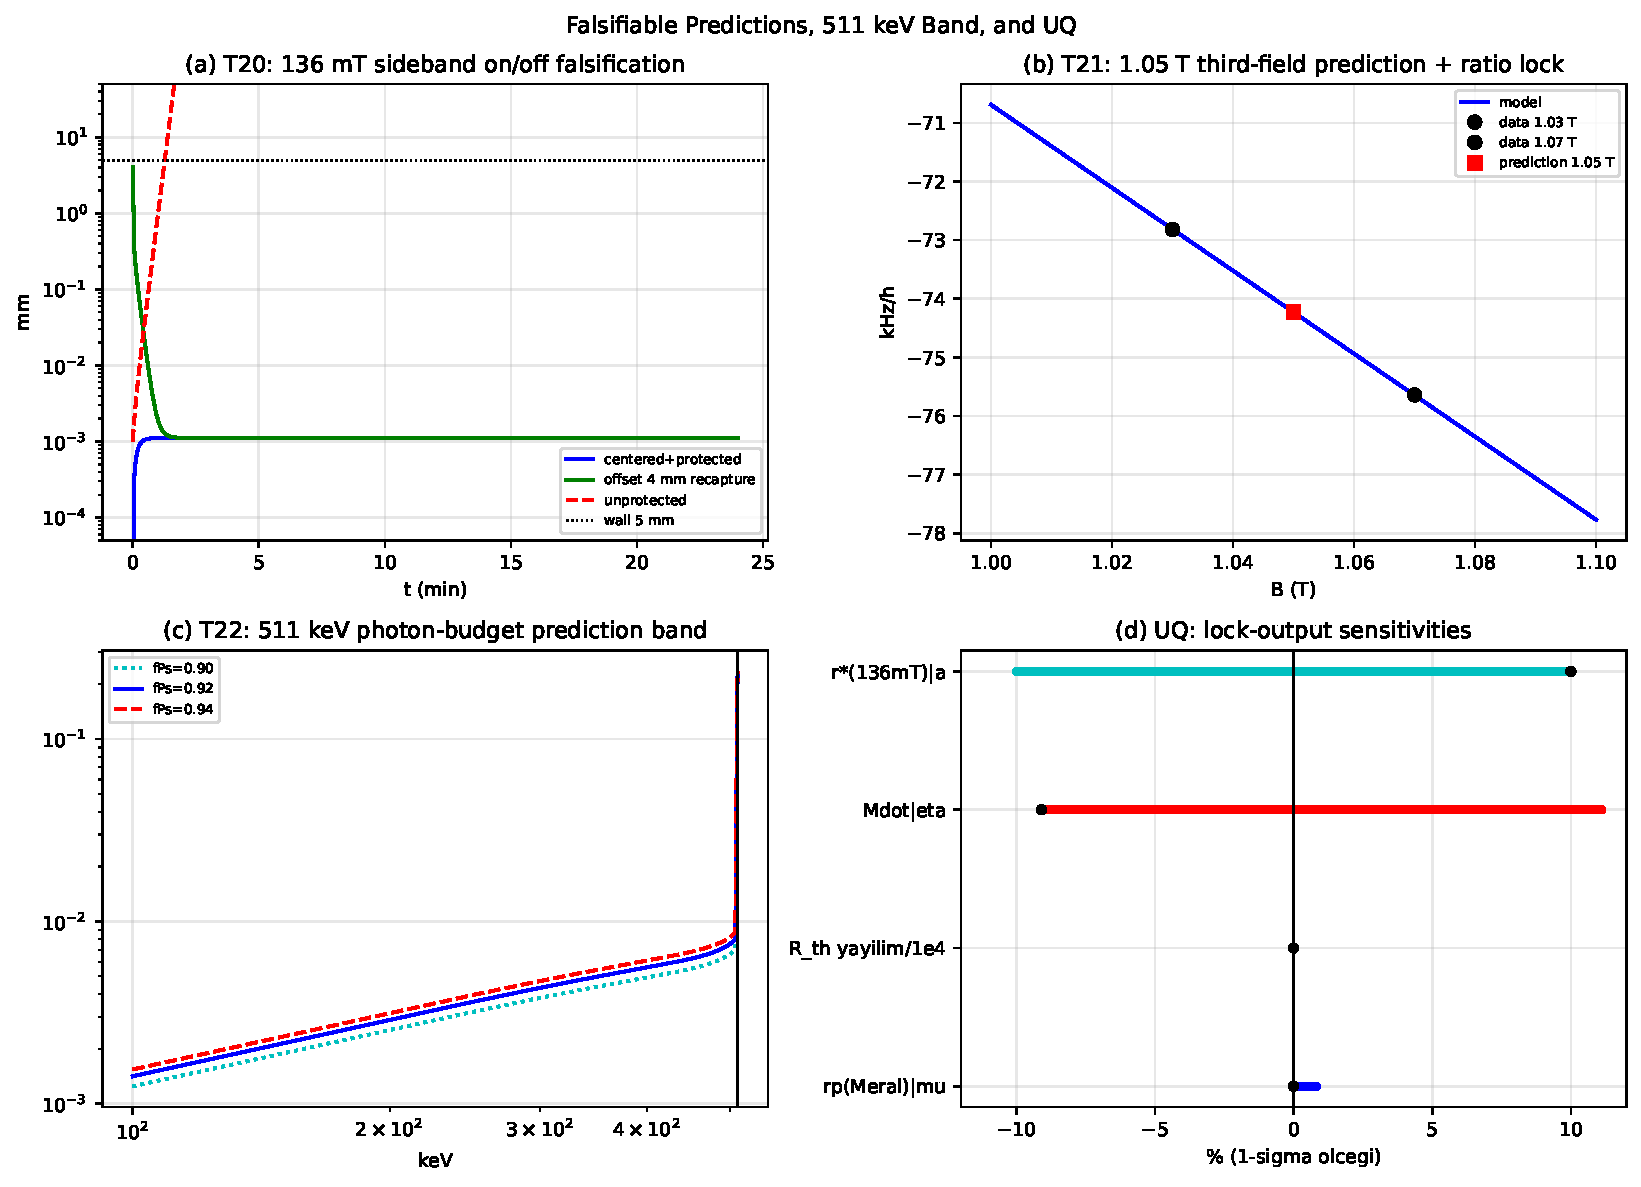
\includegraphics[width=\textwidth]{../figs/fig10_falsifiable_predictions_UQ_en.pdf}
\caption{\textbf{Falsifiable predictions, 511 keV band, and UQ (2$\times$2):} (a) T20 136 mT sideband on/off falsification (offset recapture vs.\ unprotected wall loss), (b) T21 1.05 T third-field prediction and ratio lock, (c) T22 511 keV photon-budget prediction band ($f_{\mathrm{Ps}}=0.90/0.92/0.94$), (d) UQ lock-output sensitivities.}
\label{fig:fig10}
\end{figure}

\clearpage

\section[Conclusion, Verification Summary, and Reproducibility]{Conclusion, Verification Summary, \\ and Reproducibility Instructions}

Theorem VIII closes the series' falsification ring: the 136 mT sideband pair (Table~\ref{tab:t20}), the 1.05 T third-field prediction (Table~\ref{tab:t21}), the 511 keV photon-budget band (Table~\ref{tab:t22}), and UQ (Table~\ref{tab:uq}) are pre-registered, refutable numbers. The numerical chain closes at \texttt{T1--T22 (22/22 PASS)}; the independent mini-solver gives \texttt{7/7 PASS}.

\subsection*{Data and Code Availability (Reproducibility Instructions)}

The open-source computational physics solver was developed in \textbf{Stationary Strings Theorem V [5]} (\texttt{stationary-strings-v} repository, \path{duran_sicimler_sim/solver_engine.py}); the Phase 6 (\texttt{Tests T20--T22} + UQ) verification routines and the Figure~\ref{fig:fig10} generator (\path{duran_sicimler_sim/generate_figures.py}) ship inside the same open-source solver engine. The independent cross-check (\path{duran_sicimler_sim/mini_check_viii.py}) never imports the solver. Readers can independently run and verify all 22 tests and Figure~\ref{fig:fig10} from scratch with:
\begin{quote}
\small
\texttt{python} \path{duran_sicimler_sim/solver_engine.py} \\
\texttt{python} \path{duran_sicimler_sim/mini_check_viii.py} \\
\texttt{python} \path{duran_sicimler_sim/generate_figures.py}
\end{quote}

\begin{thebibliography}{99}
    \bibitem{meral1} Meral, F. (2025a). \textit{Stationary Strings Theorem: Rebirth of Perfect Order in the Absence of Time and Entropy}. Open-source package: \texttt{stationary-strings-i} (\url{https://github.com/fahrim/stationary-strings-i}).
    \bibitem{meral2} Meral, F. (2025b). \textit{Stationary Strings Theorem II: Relativity, Phase Transition, and the Cosmological Cycle of Information}. Open-source package: \texttt{stationary-strings-ii} (\url{https://github.com/fahrim/stationary-strings-ii}).
    \bibitem{meral3} Meral, F. (2026a). \textit{Stationary Strings Theorem III: Two-Dimensional Duality of Matter, Vortex Singularity, and Phase Separation into Information}. Open-source package: \texttt{stationary-strings-iii} (\url{https://github.com/fahrim/stationary-strings-iii}).
    \bibitem{meral4} Meral, F. (2026b). \textit{Stationary Strings Theorem IV: Cosmic Fission, Vortex Fuel, and the Singularity-Free Information Core}. Open-source package: \texttt{stationary-strings-iv} (\url{https://github.com/fahrim/stationary-strings-iv}).
    \bibitem{meral5} Meral, F. (2026c). \textit{Stationary Strings Theorem V: Arresting the Navier--Stokes Vortex Singularity by Elastic String Tension}. Open-source solver package: \texttt{stationary-strings-v} (\url{https://github.com/fahrim/stationary-strings-v}, \path{duran_sicimler_sim/solver_engine.py}).
    \bibitem{meral6} Meral, F. (2026d). \textit{Stationary Strings Theorem VI: Dirac--Majorana Chiral Peeling, the $\Lambda_{\mathrm{Meral}}$ Constant, and CERN Synthesis}. Open-source package: \texttt{stationary-strings-vi} (\url{https://github.com/fahrim/stationary-strings-vi}).
    \bibitem{meral7} Meral, F. (2026e). \textit{Stationary Strings Theorem VII: Self-Consistent Vortex Saturation in CERN ALPHA Traps, Lineshape, and the Ore--Powell Resolution}. Open-source package: \texttt{stationary-strings-vii} (\url{https://github.com/fahrim/stationary-strings-vii}).
    \bibitem{akbari2025} Akbari, R. \textit{et al.} (ALPHA Collaboration). (2025). Be$^+$ assisted, simultaneous confinement of more than 15000 antihydrogen atoms. \textit{Nat.\ Commun.\ \textbf{16}}, 10106. \url{https://doi.org/10.1038/s41467-025-65085-4}
    \bibitem{alpha2026} Akbari, R. \textit{et al.} (ALPHA Collaboration). (2026). Four ppm measurement of the antihydrogen ground-state hyperfine splitting. \textit{Nature} \textbf{653}, 1022--1026. \url{https://doi.org/10.1038/s41586-026-10556-x}
    \bibitem{siegert2026} Siegert, T. \& Yoneda, H. (2026). On the Possibility of an Extragalactic Positron Annihilation Signal. \textit{A\&A}, accepted. \url{https://arxiv.org/abs/2605.21289}
    \bibitem{yoneda2025} Yoneda, H., Siegert, T. \& Mittal, S. (2025). Imaging the positron annihilation line with 20 years of INTEGRAL/SPI observations. \textit{A\&A} \textbf{702}, A220. \url{https://arxiv.org/abs/2509.01066}
    \bibitem{base2026} Leonhardt, M., Morgner, J. \textit{et al.} (BASE Collaboration). (2026). Road transport of trapped antiprotons. \textit{Nature} \textbf{657}, 906--911. \url{https://doi.org/10.1038/s41586-026-11019-z}
    \bibitem{ore1949} Ore, A. \& Powell, J.~L. (1949). Three-photon annihilation of an electron-positron pair. \textit{Phys.\ Rev.\ 75}, 1696--1699.
    \bibitem{pestieau2002} Pestieau, J. \& Smith, C. (2002). Soft photon spectrum in orthopositronium and vector quarkonium decays. \textit{Phys.\ Lett.\ B524}, 395--399.
    \bibitem{planck2018} Planck Collaboration. (2020). Planck 2018 results. VI. Cosmological parameters. \textit{A\&A} \textbf{641}, A6. \url{https://arxiv.org/abs/1807.06209}
    \bibitem{breit1931} Breit, G. \& Rabi, I.~I. (1931). Measurement of nuclear spin. \textit{Phys.\ Rev.\ 38}, 2082--2083.
    \bibitem{churazov2005} Churazov, E., Sunyaev, R., Sazonov, S. \textit{et al.} (2005). Positron annihilation spectrum from the Galactic Centre region observed by SPI/INTEGRAL. \textit{MNRAS} \textbf{357}, 1377--1386.
    \bibitem{weidenspointner2006} Weidenspointner, G., Knoedlseder, J., Jean, P. \textit{et al.} (2006). The sky distribution of 511 keV positron annihilation line emission as measured with INTEGRAL/SPI. \textit{A\&A}, ESA SP-622, 25--32.
    \bibitem{jean2006} Jean, P., Knoedlseder, J., Gillard, W. \textit{et al.} (2006). Spectroscopy of the positron annihilation emission. \textit{A\&A} \textbf{445}, 579--589.
\end{thebibliography}

\end{document}
